Typically, a computational campaign for drug discovery explores a large
number of drug candidates by running several workflows multiple times, each
requiring thousands of concurrent simulations. Before embarking on a campaign
that will utilize 150 million core hours on NCSA Blue Waters, we perform
experiments to characterize the weak and strong scaling performance of HTBAC
and its overheads on Blue Waters. We validate the results of the free energy
calculations produced using HTBAC against published results.

Given that protocols like TIES are more computationally demanding than
protocols like ESMACS, it is paramount to use resource efficiently,
especially for campaigns that have a predefined computational budget. As
described in Sections~\ref{sec:science-drivers} and~\ref{sec:htbac}, adaptive
simulation methods have the potential to reduce the number of simulations
without a loss in accuracy and with a lower computational load. We run
experiments with an adaptive implementation of TIES in HTBAC, measuring the
benefits in terms of accuracy, reduced number of simulations and
computational load.

% Further, adaptive methods can also increase computational efficiency by
% improving the rate of statistical convergence and thereby reducing the time
% to solution.

% Specifying, coordinating and executing adaptive simulation methods requires
% middleware supporting runtime decisions.

% As seen in \S\ref{sec:htbac}, HTBAC has been designed to enable decisions
% based on intermediate runtime results. These results are evaluated to
% determine a redistribution of resource to better support the execution of
% new simulations. We use HTBAC to perform experiments about adaptivity,
% comparing and characterizing resource efficiency with non-adaptive
% simulation methods.

% - Weak Scalability Design : Keep Pipeline of Ensembles to show barrier
%   needed in S5 and S6.
% - Performance, generality with weak scaling (agnostic to kernel) Added
%   functionality (do not speak about binding adaptivity to performance or
%   generality).
% - In use case: add in why TIES is challenging, and why adaptivity is
%   challenging.

% \mtnote{General note. \\
%         - Currently, this section is a merge of two distinct contributions.
%           These need to be better merged. For example, we should consider
%           whether (i) the description of the adaptive experiments should be
%           moved to the first subsection ``Experimental Setup''; (ii) Table 1
%           should be extended to include the adaptive/nonadaptive properties;
%           (iii) the discussion of the results should have a uniform
%           argumentative format; etc.\\
%         - The structure of the section should be revise making the division
%           in subsections consistent and changing/refining their naming.\\
%         - A.0,1,2 require major rewriting of the text and the writing of
%           relevant portions of new text. This includes: (i) eliminating
%           redundant (copied) text; (ii) Eliminating or referencing text
%           copied from other publications; (iii) reorganize the argumentation
%           following the other general note left in the comments and better
%           separating the experimental variables (especially including
%           adaptive/nonadaptive) properties; (iv) adding plots (even if with
%           incomplete results) and writing an actual analysis of the results
%           for each plot.}


% \jdnote{Revisions: \\ 
%         - Rewrote experimental setup by starting with motivation and
%           explaining overview of experiments
%         - Appended all experiments to table
%         - Created subsections for weak scaling, strong scaling, validation,
%           adaptive experiments
%         - Added plots (some are incomplete) and rearranged analysis
%         - Kristof added his data for adaptive experiments and
%           wrote results 
%         - Strong scaling subsection still waiting on data from ESMACS
%         - For now, removed anything related to Titan}

% \jdnote{should we mention anything about exascale?}\mtnote{I would not but
% I would quantify the scale at which we need to run. As it stands, this
% sentence appears too generic too me.} \jdnote{mentioned lower bound on
% concurrent number of simulations}

% \mtnote{what does this mean? We cited the results already in the paper?
% These results are published?}
% \mtnote{This sentence does not read well to me. I would refine, depending
% on the answer to the previous comment}.
% \jdnote{I meant to say we validate our free energy calculation results from
% this paper with known results . Does it make more sense now?}

% \mtnote{Grammar: more than?}\jdnote{more than ESMACS}
% \mtnote{Methods for? Maybe `simulation methods'?}

% \mtnote{simulation?}
% \mtnote{simulation?} 
 
% \mtnote{Note: experiments are not adaptive, they are about adaptive
% simulation methods. Analogously, experiments are not compared to
% non-adaptive experiments but they (should) offer comparable data about both
% types of methods.} \mtnote{Note: I rewrote the whole paragraph. The
% previous version was compressed and ``left too much in the authors'
% pens''.}

% A -------------------------------------------------------------------------
\subsection{Experiment Setup}\label{ssec:exp_design}

Table~\ref{tab:experiments} shows 7 experiments we designed to characterize
the behavior of HTBAC on Blue Waters. Each experiment executes the ESMACS
and/or TIES protocol for different physical systems. Experiments 1--5 use the
BRD4 physical systems provided by GlaxoSmithKline, while experiments 6 and 7
utilize the PTP1B, MC1, and TYK2 physical systems. 
% which are a diverse set of proteins.

\begin{table*}
    \caption{Parameters of scalability and adaptivity
    experiments.}\label{tab:experiments}
    \centering
%    \resizebox{\textwidth}{!}{
    \begin{tabular}{l            % Experiment ID
                    l            % experiment type
                    l            % physical system 
    %                l            % CI
                    l            % protocol type
                    l            % number of protocols
                    l            % total cores
                    }
    %
    \toprule
    %
    \B{ID}                            &  % Experiment ID
    \B{Type of Experiment}            &  % experiment type
    \B{Physical System(s)}            &  % physical system
    % \B{Computing Infrastructure (CI)} &  % CI
    \B{Protocol(s)}                   &  % protocol type
    \B{No. Protocol(s)}               &  % number of protocols
    \B{Total Cores}                   \\ % total cores
    %
    \midrule
    %
    \B{1}                             &  % Experiment ID
    Weak scaling                      &  % experiment type
    BRD4                              &  % physical system
    % Blue Waters                       &  % CI
    ESMACS                            &  % protocol type
    (2, 4, 8, 16)                     &  % number of protocols
    1600, 3200, 6400                  \\ % total cores
    % 
    \B{2}                             &  % Experiment ID
    Weak scaling                      &  % experiment type
    BRD4                              &  % physical system
    % Blue Waters                       &  % CI
    TIES                              &  % protocol type
    (2, 4, 8)                         &  % number of protocols
    4160, 8320, 16640                 \\ % total cores
    %
    \B{3}                             &  % Experiment ID
    Weak scaling                      &  % experiment type
    BRD4                              &  % physical system
    % Blue Waters                       &  % CI
    ESMACS + TIES                     &  % protocol type
    (2, 4, 8)                         &  % number of protocols
    5280, 10560, 21120                \\ % total cores
    %
    \B{4}                             &  % Experiment ID
    Strong scaling                    &  % experiment type
    BRD4                              &  % physical system
    % Blue Waters                       &  % CI
    TIES                              &  % protocol type
    (8, 8, 8)                         &  % number of protocols
    16640, 8320, 4160                 \\ % total cores
    %
    \B{5}                             &  % Experiment ID
    Strong scaling                    &  % experiment type
    BRD4                              &  % physical system
    % Blue Waters                       &. % CI
    ESMACS                            &  % protocol type
    (16, 16, 16)                      &  % number of protocols
    6400, 3200, 1600                  \\ % total cores
    %
    \B{6}                             &  % Experiment ID
    Non-adaptivity                    &  % experiment type
    PTP1B, MC1, TYK2                  &  % physical system
    % Blue Waters                       &  % CI
    TIES                              &  % protocol type
    (1, 1, 1)                         &  % number of protocols
    2080, 2080, 2080                  \\ % total cores
    %
    \B{7}                             &  % Experiment ID
    Adaptivity                        &  % experiment type
    PTP1B, MC1, TYK2                  &  % physical system
    % Blue Waters                       &  % CI
    TIES                              &  % protocol type
    (1, 1, 1)                         &  % number of protocols
    2080, 2080, 2080                  \\ % total cores
    %
    \B{8}                             &  % Experiment ID
    Reference                         &  % experiment type
    PTP1B, MC1, TYK2                  &  % physical system
    % Blue Waters                       &  % CI
    TIES                              &  % protocol type
    (1, 1, 1)                         &  % number of protocols
    10400, 10400, 10400                  \\ % total cores
    %
    \bottomrule
    %
    \end{tabular}
%    }
\up{}
\end{table*}

Experiment 1 and 2 measure the weak scaling of HTBAC using the ESMACS
(Experiment 1) and TIES (Experiment 2) protocols. Experiments 3 uses both the
TIES and ESMACS protocols, characterizing the weak scaling of heterogeneous
protocol executions. Experiments 4 and 5 measure the strong scaling of
HTBAC using a fix number of instances of the ESMACS (Experiment 4) and TIES
(Experiment 5) protocols. Experiments 6--8 characterize nonadaptive and
adaptive simulation methods using the TIES protocol.

% We leverage strong scaling to support the objective in this work, which is
% to characterize: (a) the time-to-solution differences between adaptive and
% nonadaptive methods; (b) the increase in the number of resources as
% required by the nonadaptive method to reach an acceptable accuracy
% threshold. As such, we do not run an experiment about strong scaling with
% both the TIES and ESMACS protocols.

In each weak scaling experiment (1--3), we keep the ratio between resources
allocated and protocol instances constant. Consistently, for each experiment
we progressively increase both the number of cores (i.e., measure of
resource) and the number of protocol instances by a factor of 2. In each
strong scaling experiment (4--5), we change the ratio between resources
allocated and the number of protocol instances: we fix the number of protocol
instances and reduce the number of cores by a factor of 2.

Weak scaling experiments provide insight into the size of the workload that
can be executed in a given amount of time, while strong scaling experiments
show how the time duration of the workload scales when adding resources. For
all the weak and strong scaling experiments we characterize the overheads of
HTBAC, EnTK and RP, and we show an approximation of the time taken by the
resources to become available. This offers insight about the impact of HTBAC
and its middleware on the time to completion of each workload.

For weak and strong scaling experiments, we reduced the number of time-steps
of the protocols and omitted the analysis steps $S5$ and $S6$ of their
workflows (Fig.~\ref{fig:ties_esmacs_application}). These simplifications
are consistent with characterizing scalability performance instead of
simulation duration. For the experiments 1--5 we used the following
time-steps: $S1=1000$; $S2=5000$; $S3=5000$; and $S4=50000$.

We measure the following durations for Experiments 1--5:
\begin{itemize}
    \item \textbf{Total Task Execution Time}: Time taken by all the
    task executables to run on the computing infrastructure.
    \item \textbf{HTBAC Overhead}: Time taken to instantiate HTBAC, and
    validate and process the application description.
    \item \textbf{EnTK and RP Overhead}: Time taken by EnTK and RP to manage
    the execution of tasks.
    \item \textbf{\texttt{aprun} Overhead}:  Time taken by \texttt{aprun} to
    launch tasks on Blue Waters.
\end{itemize}

Note that once RP relinquishes the control flow to \texttt{aprun}, the
precise time at which \texttt{aprun} schedules each task on a compute node
and the MD kernel of each task begins execution cannot be measured. Instead,
for each task, we measure the difference between the task execution time and
its \texttt{NAMD} kernel execution time, provided by the \texttt{NAMD} output
logs. In this way, we approximate the time taken by \texttt{aprun} to launch
the task. Once aggregated, these measures constitute what we defined as
\texttt{aprun} Overhead.

Experiments 6--8 compare the accuracy and time to solution of nonadaptive and
adaptive simulation methods. For the nonadaptive simulation method of
Experiment 6 we use 13 preassigned and approximated $\lambda$ windows,
consistent with the value reported in Ref.~\cite{Bhati2017}. In this way, we
produce 65 concurrent simulations for stages $S1$--$S4$ of TIES (see
Fig.~\ref{fig:ties_esmacs_application}). The production simulation stage $S4$
executes each simulation for \SI{4}{\nano\second}. Stage $S5$ has 5 analysis
tasks which aggregate the simulation results of $S4$. The global analysis
stage $S6$ has a single task that aggregates the results from $S5$.

In the adaptive implementation~\ref{fig:adaptive_TIES}, we initialize the
TIES protocol with 3 $\lambda$ windows, obtaining 15 replicas. We separate
stage $S4$ of each TIES replica into 4 sub-stages. Each sub-stage runs a
\SI{1}{\nano\second} simulation, followed by an adaptive quadratures analysis
which estimates free energy errors with respect to each interval of two
$\lambda$ values.

% We evaluate the total number of $\lambda$ windows as
% determined by the adaptive quadrature results in order to measure the
% differences in time duration between adaptive and non-adaptive methods as
% well as the differences in accuracy.

We use Experiment 8 to compare the adaptive and non-adaptive execution of
TIES. We use a large number of (65) equally spaced $\lambda$ windows to
calculate the free energy with high accuracy. This creates a baseline
against which to compare the adaptive and non-adaptive results.

\begin{figure}
  \centering
  \includegraphics[width=\columnwidth]{figures/Adaptive_TIES.pdf}
  \caption{Adaptive workflow for TIES. After equilibrating 3 
  $\lambda$, the first stage starts. This is followed by analysis at every
  $\lambda$ interval, to decide whether to add a new window in between. In
  our implementation, the simulation-analysis cycle is repeated for 4
  simulation steps, not shown here.}\label{fig:adaptive_TIES}
\up{}
\up{}
\up{}
\end{figure}

We assigned the following simulation time-steps in Experiment 6 and 8:
$S1=3000$; $S2=50000$; $S3=50000$; and $S4=2000000$. The adaptive simulation
of Experiment 7 uses the same time-steps, apart from $S4$ which is divided
into 4 sub-stages of 500000 time-steps each.

We performed all the experiments on Blue Waters, a 26868 node Cray XE6/XK6
SuperComputer with peak performance of 13.3 petaFLOPS managed by NCSA.
consistent with NCSA policies, we initiated the experiments from a virtual
machine outside NCSA, avoiding to run persistent process on the NCSA login
node. We used HTBAC 0.1, EnTK 0.6, and RP 0.47 and the \texttt{NAMD-MPI} MD
kernel, compiled according to the capabilities of each environment and of
\texttt{NAMD} itself, and launched via the \texttt{aprun} command. For the
analysis stages in the TIES protocol we used \texttt{AmberTools}.

NCSA sets a system policy on the maximum number of processes that
\texttt{aprun} can spawn, limiting the number of concurrent tasks we can
execute on Blue Waters to $\approx$450. During the execution of Experiment 2,
we observed failing tasks with 8 TIES protocol instances, i.e., 520
concurrent tasks. In a trial of 10 repetitions at this scale, we observed an
average of $70\pm6.67$ failing tasks.% , and range of 59--83 tasks. 
More data would be required to model the distribution type of these results.

NCSA allows to run only one MPI application for each compute node. Thus, we
had to run each MD simulation with 32 cores (i.e., one compute node) even if
our performance measurement of \texttt{NAMD} on Blue Waters indicated that 16
cores would offer the best trade-off between computing time and communication
overhead.

% \mtnote{I had to simply this paragraph a lot. Please check whether I
% omitted some essential detail or got the algorithm wrong.}
% \jdnote{it works}

% \mtnote{For quality reasons, it would be better to use figures in pdf
%   format.}\jdnote{addressed}.

% \jdnote{should we mention relationship between ns and time-steps?}

% \jdnote{Should we include the scalability plot of
% a single NAMD task using aprun?}

% \mtnote{The following paragraphs are disconnected from the previous ones.
% We need a `joining' paragraph starting from something like: ``We designed n
% experiments\ldots We used m protocols\ldots See Table o\ldots''. Moved a
% paragraph here as a starting point.}\jdnote{provided ``segway"}

% Experiment 2 measures weak scaling performance of ESMACS at higher scales,
% using ORNL Titan.
% \mtnote{Would it be better to describe weak scaling in terms of solution
% time, number of resources and problem size, as done in the following
% paragraph?}\jdnote{moved to previous para when first introducing weak
% scaling}

% of the protocols \mtnote{which protocols? So far we wrote about methods
% (but we did not specify what type of methods are we referring to)}
% \jdnote{Does the modified description of the protocol types in the earlier
% paragraph give enough insight?} \mtnote{required by what/whom? ``keeping
% the number of pipelines fixed at the number required by \ldots'' or
% something like that?} \jdnote{I've changed this description of ws, do this
% sentence and the next suffice?}

% By design of each protocol, an increase in the number of instances means an
% increase in the number of pipelines. Further, \jdnote{mention the
% relationship between protocols and pipelines in section IV.}

% \mtnote{property of? I would replace with: ``weak scaling provides
% insight\ldots''} provides insight

% Next, we measure strong scaling performance of the ESMACS and TIES
% protocols in experiments 4 and 5, respectively, by fixing the number of
% protocol instances, but reducing the cores by a factor of 2 in each run.

% \mtnote{which ones?} by fixing the workload i.e. \mtnote{Grammar: please be
% careful about the use of `i.e.' as explained in my previous set of
% comments}
% \mtnote{Why do we need the `i.e.' at all? What does `workload' add?
% ``\ldots by fixing the number of pipelines of each protocol and reducing
% \ldots''}
% \jdnote{also changed this description of ss.}

% the number of cores by a factor of 2 in each run.

% \mtnote{what does `timing' mean in this context? Duration? }
% \jdnote{will be defined in section IV}\mtnote{we will define
% `what'?}\jdnote{ignore earlier comment, the correct phrasing is time
% duration of the workload, but I am not sure if this causes
% confusion}\jdnote{ also workload will be defined in Section IV}

% \jdnote{expecting linear speedup, and expect fixed overheads}\mtnote{is
% this comment about text that still needs to be written? If so, I would not
% mention expectations of results in the design section.}

% \mtnote{of?}\jdnote{addressed}

% Experiments 4 measures the strong scaling performance of ESMACS while
% experiment 5 repeats the same strong scaling experiment using the TIES
% protocol.

% \mtnote{This is a placeholder for an actual paragraph: note how the
% previous paragraphs have a structure based on numbering experiments (and
% referring them to the table via references that are still missing), while
% this and the following paragraphs do not use the same structure. Please
% expand as needed and note that a section is not `ready' until this kind of
% uniformity is not achieved.}\jdnote{I've added experimental design of
% adaptive/nonadaptive methods.}

% Keep iterating on the next two paragraphs to get the right description from
% Kristof

% We perform the experiments for the nonadaptive (experiment 6) and adaptive
% (experiment 7) simulation methods with the same number of cores and
% simulation duration (Table~\ref{tab:experiments}). By fixing these
% parameters, we enable the comparison between the accuracy and time to
% solution of the two methods.

% By design of the nonadaptive TIES workflow
% (Fig.~\ref{fig:ties_esmacs_application}), each $\lambda$ window creates a
% new simulation condition that must be replicated. TIES requires 5 replicas
% per $\lambda$, thereby producing $\lambda \times 5$ or simulations.

% \mtnote{Reference table and exp number}
% \jdnote{addressed in this and previous sentence}
% \mtnote{Reference table with S*}
% \jdnote{the ref to Fig.~\ref{fig:ties_esmacs_application} already points
% to the description of S*, no?}
% \mtnote{Grammar: no spaces before and after dashes}
% \jdnote{noted}
% \jdnote{reworded this paragraph}

% \mtnote{Grammar: it is not clear to what this `this' refers to} produces a
% total of 65 concurrent simulations for stages $S1$--$S4$ \mtnote{Reference
% table with S*} \mtnote{Grammar: no spaces before and after
% dashes}\jdnote{noted}. The production simulation stage $S4$ executes each
% simulation for 4ns. The analysis stage $S5$ assigns 5 analysis tasks which
% aggregate simulation results of $S4$ with respect to each replica. The
% global analysis stage $S6$ contains a single task that aggregates the
% results from $S5$.

% \mtnote{different from what?}\jdnote{changed}

% The estimation of the error determines whether
% \mtnote{Grammar: as already commented in the previous draft, `whether'
% implies already `or not'.\jdnote{noted} Adding it is
% redundant.}\jdnote{noted} to spawn additional $\lambda$ windows. If the
% error estimate in a certain interval is higher than the acceptable
% threshold, a new $\lambda$ window is assigned halfway between the interval.
% If the critical threshold is reached, we have reached convergence and the
% application stops; else, current simulations continue executing and new
% simulations begin executing based on newly generated $\lambda$ windows.

% The estimation computation \mtnote{This is too compressed. In itself,
% `estimation computation' means little. The reader has to go back to the
% previous paragraph to understand what those two words refer to. `We compute
% the free energy errors\ldots'?} is captured \mtnote{`captured' is
% metaphorical. Metaphors should be avoided when writing science. Also, the
% sentence is passive and also this should be avoided in scientific writing}
% as a single stage \mtnote{Does the reader know what a stage is?} containing
% a single task. By design of the adaptive quadrature algorithm \mtnote{where
% this algorithm is used? Does the reader know about it?}, the number of
% additional $\lambda$ windows will vary across candidates, which will impact
% the number of simulation-analysis iterations. \mtnote{And\ldots We are
% missing an explanation of why this is important from an experimental design
% point of view. Maybe because it changes the number of tasks?}
% \jdnote{will call this something else}.\jdnote{check with Kristof on the
% local and global analysis that happen for nonadaptive}

% \mtnote{Note: paragraphs like this indicate lack of iteration before
% releasing the manuscript for review. Too much is assumed, too little is
% converted from thoughts to written form. How the academic writing process
% works: Before releasing the manuscript for review, the author goes back and
% forth across the manuscript multiple times. Progressively, each paragraph
% is iterated until it is grammatically correct and it stands on its own
% content-wise. When a manuscript is received for review, the reviewer focus
% on the content of each paragraph and section, assessing their completeness
% and conceptual/formal correctness. Each grammatical error, each
% inconsistency or missing detail distracts the reviewer impeding her
% work.}\jdnote{I've removed the previous paragraph that gave trouble and
% updated the experimental setup of the adaptive and non-adaptive methods.}

% This procedure is repeated until convergence, at which point all concurrent
% simulation are terminated. We define convergence as the point in the
% production-analysis loop at which a desired error threshold is reached.

% When one protocol has converged whilst another has not, we can shift
% computational resources to favor simulations that require additional
% resources.

% individual\mtnote{I am not sure I understand what individual means in this
% context}

% strong scaling performance of ESMACS and TIES on Blue Waters. We fix the
% number of protocols and vary the amount of resources in order to produce
% generations

% \mtnote{The reader will struggle to understand what `generations' means in
% this context.} of execution.
% \mtnote{Two sizable paragraphs to describe weak scaling, four lines to
% describe strong scaling? I would expand.}

% \mtnote{This sentence seems to suggest that we run our experiments on a
% virtual machine. I know what you mean but the average reader has no idea
% about the capabilities of our middleware and the policies of not executing
% persistent processes on the head node of Blue Waters.}
% \jdnote{Can we omit this sentence?}

% and the Titan ones from an ORNL login node. as Blue Waters does not permit
% executing applications directly on the login node. The ORNL Titan
% experiments had instead to be performed from an ORNL login node.

% The minimization tasks of $S1$ to 1000 simulation time steps, while the
% equilibration tasks in $S2$ and $S3$ are \mtnote{Grammar: inconsistent
% tense. `Were' or `assign'} assigned 5000. The MD simulation tasks in $S4$
% are assigned 50,000 steps.

% \mtnote{when/why a simulation task is `production'? I am not sure I
% understand what that means}\jdnote{removed production for weak/strong.
% Production applies to adaptive/nonadaptive which need to show the
% production scale timesteps i.e. 2 or 3M}

% while on Titan a non-MPI, multi-core NAMD engine. On Titan we compiled NAMD
% with CUDA for the ESMACS experiments, and with OpenMP for the for TIES ones
% as NAMD does not support alchemical perturbations execution on GPU.

% application launch method, which is the NCSA Blue Waters designated command
% for describing the application parameters and resource requirements
% \mtnote{does the reader know what is a launch method?} \jdnote{better?}
% \mtnote{Unfortunately not: https://bluewaters.ncsa.illinois.edu/using-aprun
% . Alternative: `We perform (or performed depending on what tense you will
% decide to use) all Blue Waters experiments using the \texttt{aprun} command
% to launch the MD simulations'}.
% \jdnote{noted and addressed.} During our scalability experiments we found
% two main limitations.
% \mtnote{this is too generic. Based on this paragraph, we found two main
% limitations. This is what we should therefore write.}

% \jdnote{I've changed this again because the limitation on the max no. of
% concurrent CUs is a system setting (similar to what we experienced
% first-hand on Titan), but it's not a technical limitation of APRUN.}

% Unfortunately, \texttt{aprun} has several \mtnote{this is too generic.
% Based on this paragraph, we found two main limitations. This is what we
% should therefore write.} limitations: First, the number of concurrent tasks
% execution is limited to \ldots. On average, during our experiments we were
% not able to execute more than 436 concurrent tasks.
% \mtnote{how do we know this average?}.
% \jdnote{would it make sense to show a bell curve of the distribution of
% failing units? I have 8 data points, but I can run more and include Mark's
% Cray paper?}
% \mtnote{Agreed. The comment was about saying that you observed this average
% while performing experiments. See how I rewrote the paragraph}.
% \jdnote{added the data for the failing units however including a
% distribution of this data is not meaningful as the sample size in the
% number of trials is very small. By looking at some histograms where I vary
% the bin size, it could be either Gaussian or multimodal distribution. Only
% more data will tell us for sure what kind of distribution we have.
% Moreover, Mark's Cray paper shows range of concurrent units using ORTE-LIB,
% so I will not reference this here.}

% \mtnote{this is metaphorical. Please change using a factual predicate.}
% \jdnote{changed the phrasing a bit}
% \mtnote{Note: I had to rewrite the paragraph because the current version
% was too unrefined. Please see the note above about the need to
% progressively refine each paragraph.}

% From our own scalability performance measurements of NAMD on Blue Waters,
% we observe the ideal cores per task to be 16, however Blue Waters does not
% permit running multiple MPI applications on the same node, hence each NAMD
% task requires a complete node to maintain concurrency.
% \mtnote{This needs to go before previous sentence as it explains why we use
% 32 cores for each NAMD executable. Note: it is not true that NAMD
% `requires' 32 cores as stated above.}\jdnote{moved here since this para
% discusses \texttt{aprun} limitations}

% In order to continue execution on higher scales \mtnote{Why do we need an
% higher scale?}, we perform higher scales \mtnote{I am not sure what
% `performing higher scales' means} on ORNL Titan, using the ORTE launch
% method \mtnote{Why don't we use ORTE on BW? The reader will probably know
% that they are similar machines}.

% The difference in platforms produces overheads \mtnote{Only overheads or
% also different execution time of NAMD---seeing the differences described in
% the previous paragraph} that can be captured by RTS \mtnote{does the reader
% know what a RTS is?} and are shown \mtnote{careful with the use of
% `demonstrate', especially in a scientific paper} in the figures
% \mtnote{which figures?} as "APRUN overhead" and "ORTE overhead"
% \mtnote{LaTeX requires different quotes}.

% For tasks pertaining to $S1$ -- $S4$ \mtnote{What are $S1$ and $S4$? LaTeX
% wants double dash without space to indicate a range}, while the analysis
% stage, $S5$ use AmberTools \mtnote{grammar: I am not able to parse this
% sentence}.

% For both adaptive and nonadaptive experiments \mtnote{the reader knows
% about Experiment 1-7, not about adaptive/nonadaptive ones},

% In the nonadaptive experiments,

% For the adaptive experiments, each substage
% \mtnote{What is a `substage'?} of $S4$ i.e. $S4.1$--$S4.4$ is assigned
% 50,000 steps.\mtnote{Why the difference is number of steps and why it is
% relevant?}

% HTBAC submits a resource request to EnTK, to which EnTK uses RP to acquire
% resources via a single pilot. Accordingly, we request the maximum number of
% cores required by the workload as the number of cores in a pilot.

% To characterize the weak scaling performance of TIES \mtnote{I am not sure
% I understand this sentence: For measuring the weak scaling performance of
% TIES?}
% \jdnote{better?}, we use between 4160 and 33280 cores as indicated in
% Fig.~\ref{fig:weak_scaling_TIES} because the NAMD executable used in all
% tasks \mtnote{does the reader know what a task is in this context?}
% \jdnote{will be defined in Section IV} from $S1$-$S4$ require
% \mtnote{grammar: requires} a single node i.e. 32 cores per task, as
% mentioned earlier in the APRUN limitation.
% \mtnote{why?}\jdnote{32 cores/task addressed by earlier mention of aprun
% MPI limit}

% For strong scaling performance, we fix the number of protocol instances to
% 8 instances given that we experience failing concurrency of tasks when we
% scale the workload to 8 protocols.\mtnote{why 8?} We vary the amount of
% resources as shown in Fig.~\ref{fig:strong_scaling_TIES} by showing
% reducing of resources by a factor of 2. \mtnote{Please expand indicating
% and justifying the the chosen amount of resources. Experiments can be
% design in many ways, we need not only to describe but also to justify why
% we choose a specific design for our experiments.}\jdnote{better?}

% For the TIES protocol, each pipeline \mtnote{does the reader know what a
% pipeline is?}\jdnote{will be address in Section IV} consists of six stages
% \mtnote{simulation stages?}. Each of the simulation stages contains a task
% for every unique ($\lambda$, replica) combination \mtnote{does the reader
% understand this?}\jdnote{will be addressed better in section IV}. In the
% non-adaptive workflow \mtnote{we never used `workflow'. Previously we used
% non-adaptive (written as `nonadaptive') experiment. Note that we did not
% introduce adaptive/nonadaptive experiments} scenario, the first 11
% $\lambda$ windows
% \mtnote{does the reader know what a lambda window is?} consist of the
% following values: $L$ is a vector with
% \begin{flalign} L &= \{ x_i: x_i\in[0,1]\; and\; x_{i+1} = x_i + \delta \},
% where\ \delta\ is\ 0.1. %&$$L=\{ x_i: x_i\in[0,1]\; and\; x_{i+1} = x_i +
% \delta \}$$%, where $\delta$ is $0.1$.
% \end{flalign}

% We append two additional values on both ends of $L$, completing 13
% $\lambda$ windows. Each $\lambda$ window consists of five replicas.
% Therefore there are a total of 65 tasks for every simulation stage
% \mtnote{depending on the previous sections of the paper, this `therefore'
% may have to be better explained to the reader}. The production simulations
% stage, $S4$ as described in figure~\ref{fig:pst}\mtnote{missing figure}
% executes a 4 ns simulation duration \mtnote{grammar: executes a simulation
% for 4 ns? a simulation with a 4 ns duration?}. The analysis stages of the
% protocol reduce the number of tasks \mtnote{Why/how?}. The first analysis
% task consists of five tasks where each task performs an aggregate analysis
% over all $\lambda$ windows for each replica. The second analysis stage
% consists of one task that aggregates the previous results and computes a
% single average across all replicas.

% B -------------------------------------------------------------------------
% \subsection{Overhead Characterization}

% \mtnote{I would create a subsection with overheads, discussing their
% behavior and nature while referencing both weak and strong scaling
% experiments.}
% \jdnote{placing this here...}
% \mtnote{This does not work as most of the overheads are still discussed in
% the next subsection. It is getting late to keep altering the structure of
% this section. It seems to me, we are measuring: weak scaling, strong
% scaling and overheads. Do we measure and discuss overheads in both weak and
% strong scaling? If so, I would not have a separate subsection for overheads
% at this point in time from the deadline. If we are discussing them only in
% the context of the weak scaling, then we may have a problem and we need to
% discuss it.}

% We perform 5 experiments to characterize the overheads of HTBAC, EnTK,
% runtime system, and \texttt{aprun} as a function of weak and strong scaling
% properties. We compare these overheads to the total execution time of all
% the tasks, assessing the overall impact of these overheads on the
% application time to completion. We measure the following durations:

% \begin{itemize}
%     \item \textbf{Total Task Execution Time}: Time taken by the aggregate
%     of task executables to run on the computing infrastructure (CI).
%     \item \textbf{HTBAC Overhead}: Time taken to process the application,
%     instantiate HTBAC's components and subcomponents, translate protocols
%     into pipelines for EnTK, and validate resource descriptions.
%     \item \textbf{EnTK and RP Overhead}: Time taken by EnTK and its runtime
%     system (RP) to submit and manage the execution of tasks.
%     \item \textbf{\texttt{aprun} Overhead}: Approximated time taken by
%     \texttt{aprun} to launch tasks on a set of compute nodes.
% \end{itemize}

% Once the runtime system relinquishes the control flow to \texttt{aprun},
% the precise time at which \texttt{aprun} schedules each task on a compute
% node and the MD kernel of each task begins execution cannot be measured.
% Instead, for each task, we measure the difference between Task Execution
% Time and its \texttt{NAMD} kernel execution time, provided by the
% \texttt{NAMD} output logs. In this way, we approximate the portion of the
% TAsk Execution Time taken by \texttt{aprun} to launch the task. Once
% aggregated, these measures constitute what we defined as \texttt{aprun}
% Overhead.\mtnote{Am I right to assume that: $Task Execution Time = NAMD
% execution time$?}

% \mtnote{Are we sure aprun `schedules' tasks? Maybe launch as we call
% `aprun' a launch method?} \jdnote{addressed, as referenced by cray
% documentation}

% Total Time to Execution \(TTX\) measures only the aggregated execution time
% of all tasks' executables.

% \mtnote{TTX should measure only the aggregated time spent executing the
% tasks' executables. All the rest should be part of RP overhead}
% \jdnote{ This sentence doesn't need to go in but I wanted to clarify a
% point: I would like to know if we should use TTX as TTX or something else
% like Task Execution Time. We have TTX measured by events:
% \texttt{cu-exec-start} and \texttt{cu-exec-stop} , since \texttt{aprun}
% doesn't allow further scrutiny using events like \texttt{app-start} until
% \texttt{app-stop}. We use the term TTX internally, but maybe for this paper
% we should call it task execution time. TTX sounds like time to execution
% which could interpret the entire application, no?}\mtnote{I think the
% meaning of TTX depends on how it is defined. Said that, I agree we should
% avoid using the term `TTX' in this paper. I would use `tasks execution
% time' or, probably better, `total task execution time'. We want to indicate
% an AGGREGATED measure of a duration, not a measure of the time taken by a
% SINGLE task to execute. Note: this is a duration. As such, it should be an
% item of the list above, not a separate paragraph.}\jdnote{I've modified the
% descriptions}

% We characterize the execution time of all three applications \mtnote{which
% one?}, \jdnote{given that I mention what each experiment entails earlier,
% can I keep the application general and say all 3?} and overheads of HTBAC,
% EnTK, RP and \texttt{aprun}.

% \jdnote{Since we are showing overhead component separate, can we remove the
% total overhead calculation?}

% The total time to completion (TTC) of each application \mtnote{of what?}
% \jdnote{per application} \mtnote{you see the difference produced by my
% editing?} can be expressed as $TTC = TTX + T_{O}$ where Total Time to
% Execution \(TTX\) measures only the aggregated execution time of all tasks'
% executables. \mtnote{TTX should measure only the aggregated time spent
% executing the tasks' executables. All the rest should be part of RP
% overhead}\jdnote{for discussion with Matteo 06/04}\mtnote{I am afraid I do
% not understand this comment}

% % $T_{O}$ equates to the total overheads produced by HTBAC, EnTK, and % RP:
% $$T_{O} = T_{O}\textsuperscript{HTBAC} + T_{O}\textsuperscript{EnTK} + %
% T_{O}\textsuperscript{RP}$$

% \mtnote{As defined, this formula seems to add twice part of the RP
% overheads.} \jdnote{I think I'm missing something: The RP overhead is what
% I get from the pilot duration logs. Not sure where I'm duplicating} %
% \mtnote{If TTX is more than just the aggregated execution time of % all the
% tasks' executable, then TTX and $T_{O}$ both contain part of RP %
% overhead.}

% B -------------------------------------------------------------------------
\subsection{Weak Scaling Characterization}

% We investigate the weak scaling of HTBAC with three experiments: Experiment
% 1 that executes only the TIES protocol; Experiment 2 that executes only the
% ESMACS protocol; and Experiment 3 that executes both TIES and ESMACS
% together. Each experiment uses a specific protocol configuration,
% concurrently executing an increasing number of protocol instances,
% proportional to the amount of requested resources. On Blue Waters,
% \texttt{aprun} determines the upper boundary of the number of supported
% concurrent executions.

Fig.~\ref{fig:ws}(a) shows the weak scaling of HTBAC with the TIES protocol.
Each instance of the TIES protocol contains a single pipeline with 4 stages
and 65 concurrent tasks. We increase the number of protocol instances
linearly, between 2 and 8. When scaling to 8 protocol instances, we execute
more than 450 concurrent tasks, the average limit supported by
\texttt{aprun}, as described in \S\ref{ssec:exp_design}. This introduces some failures that contribute to a slight degradation in performance. 

% Nevertheless, we include results at this scale to show HTBAC's performance
% when supporting higher orders of concurrent simulations.

\begin{figure}
  \centering
    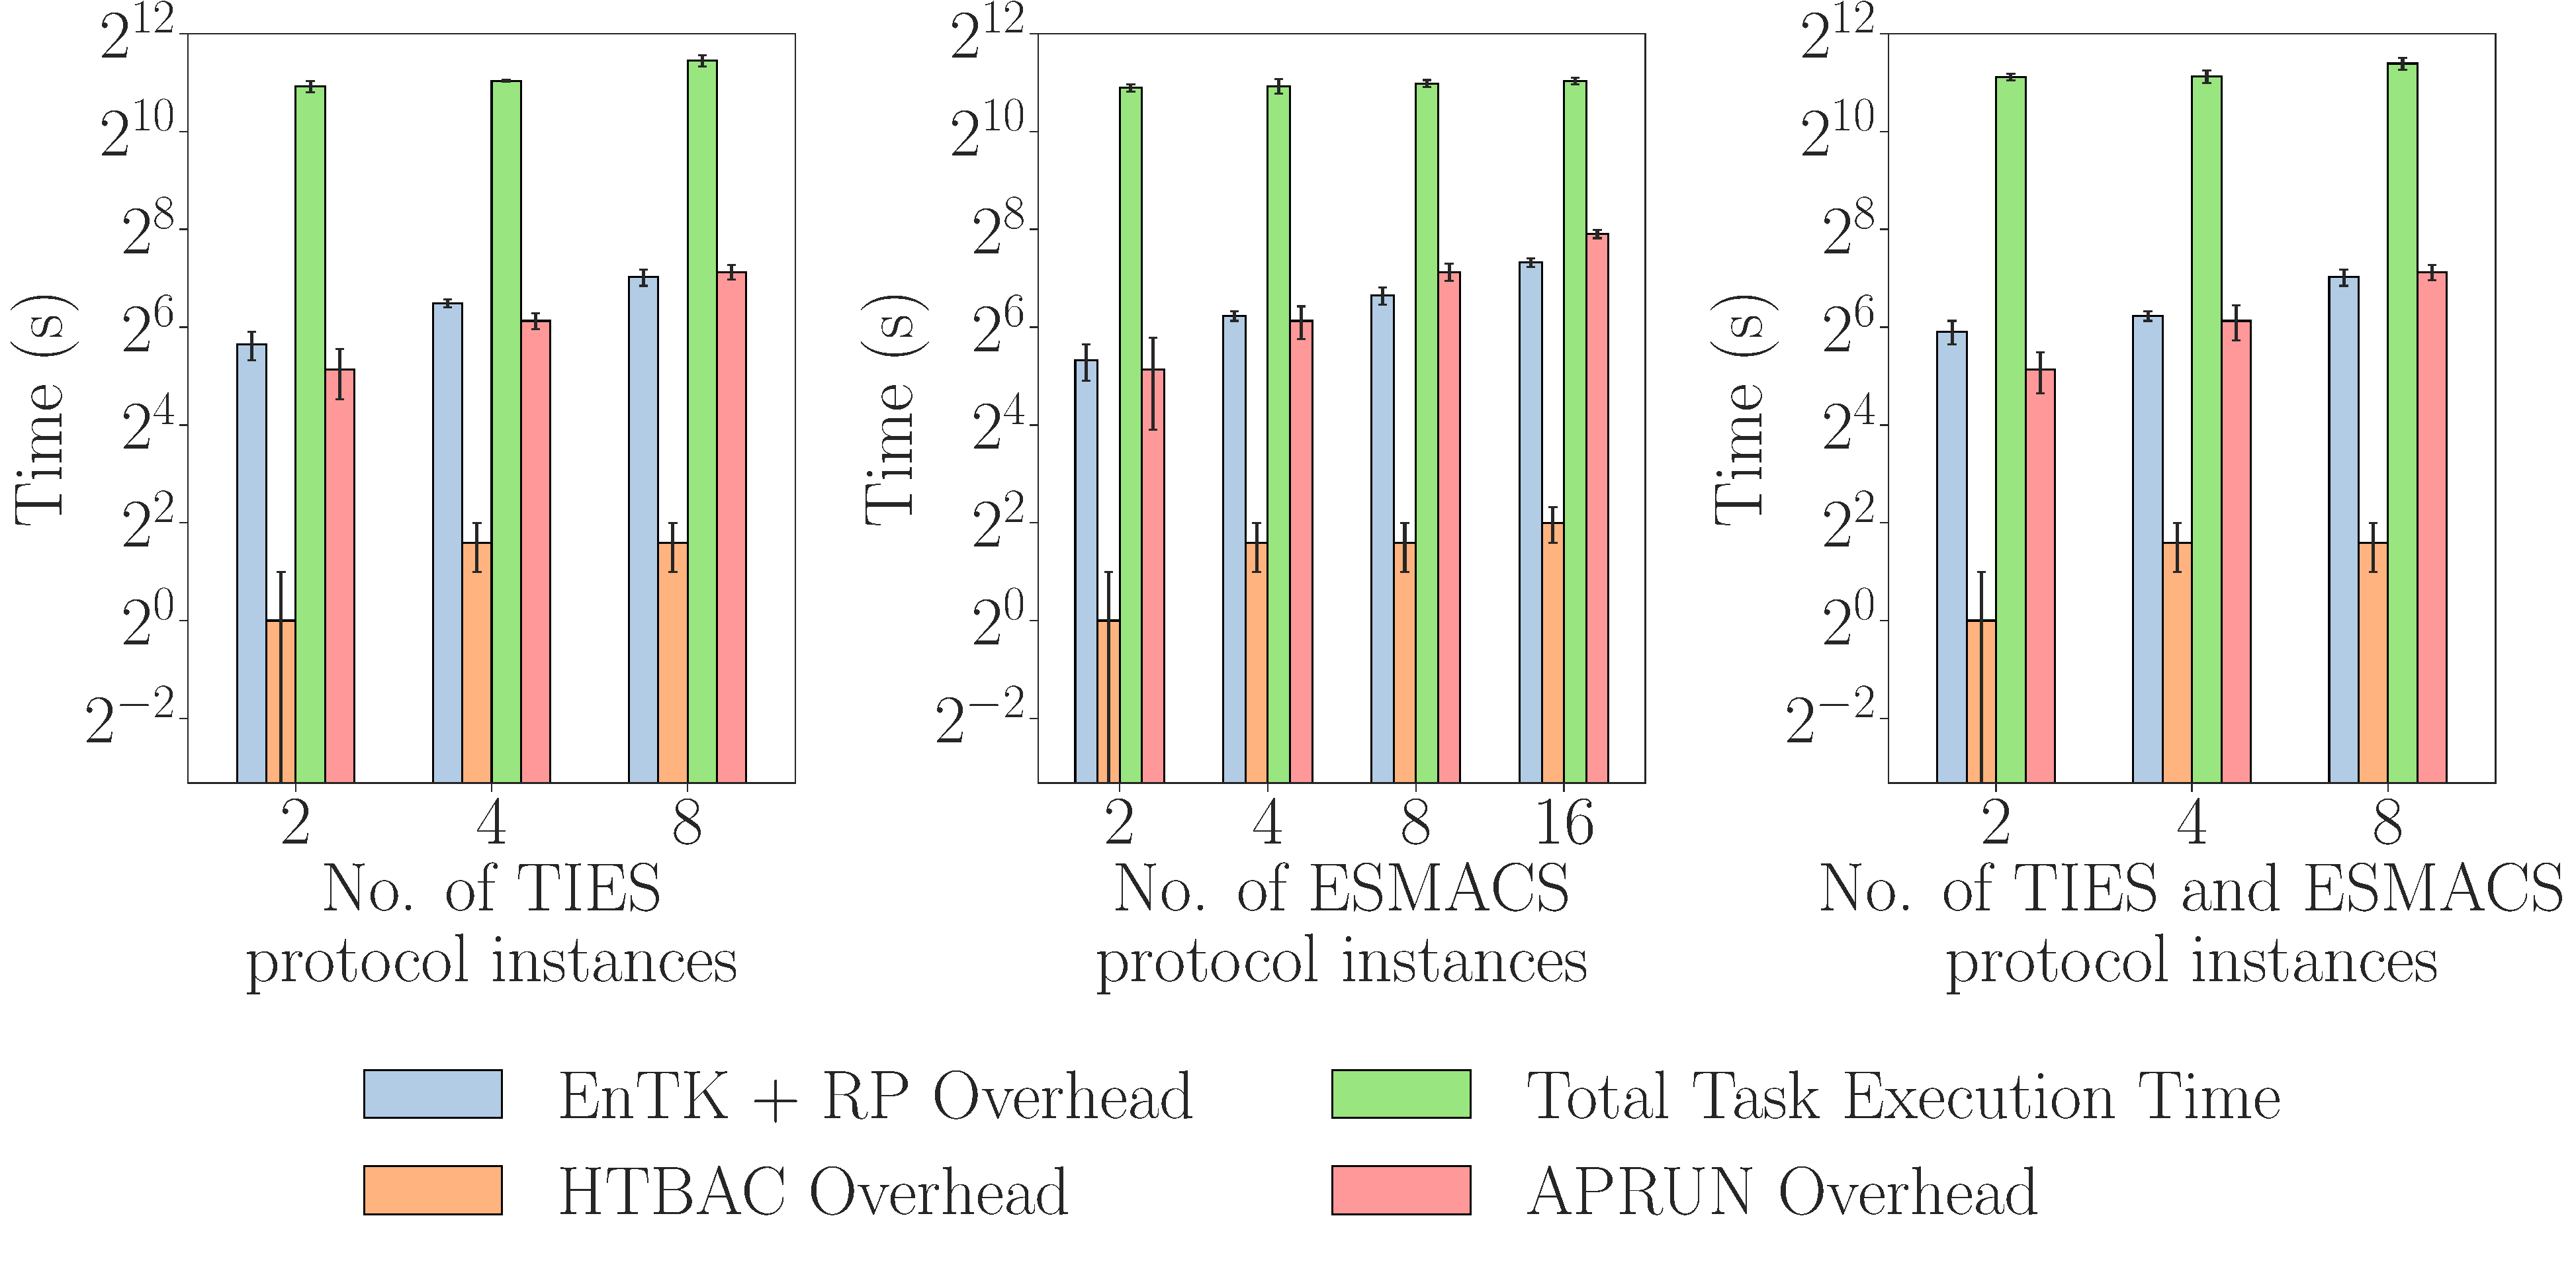
\includegraphics[width=\columnwidth]{figures/ws_all_base2.pdf}
    \caption{Weak scaling of HTBAC. The ratio number of protocol
    instances to resources is constant. Task Execution Time with and HTBAC,
    EnTK+RP, \texttt{aprun} overheads with (a) TIES (Experiment 1), (b)
    ESMACS (Experiment 2), and (c) TIES and ESMACS (Experiment
    3).}\label{fig:ws}
\up{}
\up{}
\up{}
\end{figure}

Fig.~\ref{fig:ws}(b) shows the weak scaling of HTBAC with the ESMACS
protocol. We increase the number of instances linearly, between 2 and 16.
Each ESMACS protocol contains 1 pipeline with 4 stages and 25 concurrent
tasks.

Fig.~\ref{fig:ws}(c) shows the weak scaling of HTBAC with instances of
both TIES and ESMACS protocols. Also in this case, we scale the instances of
both protocols linearly, between 2 and 8. The first configuration shows 1
ESMACS and 1 TIES protocol, and with each increase in scale we double the
number of protocols. Experiments 2 and 3 show scaling ranges within the
limit of the maximum number of concurrent tasks we can successfully execute
on Blue Waters. 

For all weak scaling experiments (1--3) we use physical systems from the
\texttt{BRD4-GSK} library with the same number of atoms and similar chemical
properties. The uniformity of these physical systems ensures a consistent
workload with insignificant variability when characterizing their performance
under different conditions.%\mtnote{moving to design?}
%
% \dwwnote{The figure captions and legends don't appear to agree which axis
% applies to which measurement. Also the legend should be inside the plots.}
% \jdnote{addressed, except with subplots I figured it would look cleaner
% with the legend at the bottom.}

In all weak scaling experiments (Fig.~\ref{fig:ws}) we observe that the value
of Total Task Execution Time (green bar) shows minimal variation as the
number of protocol instances increases. We conclude that HTBAC shows
near-ideal weak scaling behavior under these conditions.

The HTBAC overhead depends mostly on the number of protocol instances that
need to be generated for an application. This overhead shows a super linear
increase as we grow the number of protocol instances, but the duration of the
overhead is negligible when compared to Total Task Execution Time.

The \texttt{aprun} overhead increases as we approach the limit of concurrent
\texttt{aprun} processes that can be executed on Blue Waters. For example,
when scaling to 8 TIES protocol instances (Fig.~\ref{fig:ws}(a)), we see
that the increase in \texttt{aprun} overhead occurs due to task failure. This
is explained by noticing that attempts to relaunch failed tasks require
additional communication among the nodes that were running the tasks and the
MOM Nodes from which the execution is coordinated.

EnTK and RP overheads mostly depend on the number of tasks that need to be
translated in-memory from a Python object to a task
description~\cite{dakka2017,merzky2018}. As such, those overheads are
expected to grow proportionally to the number of tasks, as observed in
Fig.~\ref{fig:ws}, blue bars.

The RP overhead is calculated by measuring and aggregating the execution time
of the RP components that manage and coordinate the execution of the protocol
instances. Among these components, the task scheduler of RP introduces the
largest overhead. Due to the general scheduling algorithm loaded by default
in RP, the task scheduling overhead scales linearly with the number of tasks
that need to be scheduled.

In comparison to Total Task Execution Time, the EnTK and RP overheads are an
order of magnitude shorter, yet they directly contribute to the total
duration of the application execution. Based on Fig.~\ref{fig:ws}, we
approximate the use of our systems will results in $\approx15\%$ additional
usage of resource allocation. This overhead can be substantially reduced by
using a special-purpose scheduler for RP as illustrated in
Ref.~\cite{merzky2018}.

% \mtnote{Are we sure? In the latest RP paper I thought we wrote that the
% performance of the RP CU scheduler depends on the size of the pilot? Would
% you mind double checking?}\jdnote{sent you note on slack about discrepancy
% in papers.}\mtnote{Answered there.}

% \mtnote{protocol?}\jdnote{addressed}

% \jdnote{Maybe combine captions into 1?}\mtnote{Agreed.}\jdnote{One figure,
% 3 subplots, 1 caption is cleaner}

% The error bars are calculated using 3 trials per protocol instance measure,
% already suggesting but While it is highly desirable to use larger trials to
% determine the precision of our observations, our current data already
% suggests a trend of reproducibility.

% \mtnote{This might be considered too little without further
% explanation}\jdnote{how is this?}\mtnote{I commented it out. I believe we
% should avoid to mention how many repetitions we did altogether as we did so
% a few. Happy for this to be reverted by anyone with a more solid background
% in statistics than mine.}\jdnote{OK}

% \mtnote{total? See my previous comment about this being and AGGREGATED
% duration.}\jdnote{aggregate}

% For computational drug campaigns, efficient utilization of resources is
% most crucial consideration. In the scope of this work, we leverage the
% efficiency of resources as provided by the runtime system, in order to
% focus on scalable execution of adaptive methods that can improve accuracy
% and reduce time to solution.

% \mtnote{I am afraid this whole paragraph needed to be rewritten. I tried to
% fix it but we are missing a comparative evaluation of this overhead. For
% example, does this overhead matter when compared to TTX or TTC? Given a
% computation campaign with TIES and ESMACS, how much allocation time would
% be spent on this overhead? What would be the total percentage of
% allocation/resources spent in overheads?}\jdnote{added context}

% \mtnote{Do we `increase the number of instances linearly, between 2 and 8'
% also in experiment 2? If so, we should say that only once for Experiment
% 1--3. If not, why?}\jdnote{addressed the scaling ranges, and explained
% why}.

% \jdnote{this is to say that the fluctuations in execution times between
% data points are invariant to the physical systems}\mtnote{Nice comment, I
% would edit it and put it in the text!}.
% \jdnote{addressed}

%  \mtnote{Grammar: conjugation}\jdnote{back to the present} 

% \mtnote{does the reader know what a task is in this context?} \jdnote{will
% be defined in Section IV}

% \mtnote{grammar: I do not understand the sentence after the `;'} given by
% the sum of the constituent overheads: $$T_{O} =
% T_{O}\textsuperscript{HTBAC} + T_{O}\textsuperscript{EnTK} +
% T_{O}\textsuperscript{RP}$$.

% \mtnote{This sentence is copied from a previous paper we wrote: does the
% reader know what a CU is?}
% \jdnote{I will add in a brief mention of CU in Section IV}\mtnote{I would
% just use task as you do in the following sentence. IMHO, using CU adds yet
% another pseudo-technical term as a synonym of a term we are already using,
% i.e., task}\jdnote{noted and added reference for RP as well}
% \mtnote{Please add reference to the relevant figure(s) and details.}
% \jdnote{addressed}
% \mtnote{I commented all the following. IMHO, it does not contribute to
% understand the current analysis of the results. Do we need to expand the
% analysis?}\jdnote{It can be left out, I was just trying to explain the
% barriers in EnTK between stages that may incur on the overheads, given that
% all simulations need to finish before moving on to next stage. With
% protocols that have more tasks/stage, I thought this should be mentioned as
% a contribution.}

% \mtnote{We need to explain why TTX is affected. Are tasks restarted? Also,
% does this overhead matter? See previous comment about RP overhead impact on
% TTX/TTC/Resource utilization.}\jdnote{added a technical detail}

% \mtnote{Please refine the previous sentence as it might not say what I
% think you want to say: What does it mean that TTX is `within error margin'?
% And how this relates to `ideal weak scaling behavior'? Maybe the former
% applies to the latter instead of TTX?}.\jdnote{does this read better?}

% HTBAC enables concurrent execution of multiple protocol \mtnote{what type
% of protocols?} instances.

% ------------------------- COMMENTED BY MT -------------------------
% EnTK submits CU descriptions to a database that is then pulled by
% RP.\mtnote{I am not sure this is accurate}\jdnote{took out "same" database}
% In addition, each stage constructed by EnTK maintains sequential barriers.
% \mtnote{Doe the reader know what a barrier is?}\jdnote{I will add this to
% the EnTK description in Section IV} RP remains dormant until completion of
% the current tasks before staging the next tasks. \mtnote{This figure is
% about scaling behavior, not about the mechanics of EnTK and RP here
% discussed.}\jdnote{took out figure ref}
% ------------------------- END COMMENTED BY MT ----------------------

% The impact of the synchronization barriers increases with the number of CUs
% as seen in the 16 protocol instances data point in This pull operation
% occurs over a wide area networks, which introduces varying amounts of
% latency.

% The main contributor to the increase in overhead in RP is based on the the
% time of resources inactivity while RP schedules new tasks. As such, the
% overhead is expected to grow proportionally to the number of concurrent
% tasks~\cite{dakka2017}.

% Among these durations, the pilot duration contains the time to bootstrap
% and terminate the pilot. The task overheads contain the executor's spawning
% of the task, folder staging preparation, and operating system task
% spawning. \mtnote{We need to explain to the reader why all this is relevant
% in this context.} \jdnote{need to discuss on 06/04, should we keep these
% details or keep the focus on the paragraph just above this one?}

% \mtnote{this sentence does not read well. I would refine it}
% \mtnote{this needs further explanation}
% \jdnote{reworded paragraph, also commented out next paragraph on EnTK
% synchronization until I can justify better.}

% \mtnote{Does the reader know what aprun is? Also, I would use something
% like textttt to identify the name of a command or
% executable}\jdnote{addressed}

% \mtnote{concurrent?}\jdnote{addressed} 

% Together, the EnTK-enabled synchronization barriers and \texttt{aprun}
% overhead failures \mtnote{until now, we have implicitly assumed that our
% overheads are measured in time. Did we now use also number of failures?}
% introduce delays in the scheduling of the CUs and results in higher
% overheads \mtnote{Is this sentence circular? Overhead increases
% contributing to increasing the overhead?}. Lastly, we notice that each
% additional protocol instance contributes to roughly 55 additional seconds
% in \(TTX\).\mtnote{All this needs to be clarified and expanded into an
% actual discussion of the results.}

% We use between 4160 and 16,640 cores as indicated in
% Fig.~\ref{fig:weak_scaling_TIES}.

% To characterize the weak scaling performance of TIES \mtnote{I am not sure
% I understand this sentence: For measuring the weak scaling performance of
% TIES?}
% \jdnote{better?}, we use between 4160 and 33280 cores as indicated in
% Fig.~\ref{fig:weak_scaling_TIES} because the NAMD executable used in all
% tasks \mtnote{does the reader know what a task is in this context?}
% \jdnote{will be defined in Section IV} from $S1$ -- $S4$ require
% \mtnote{grammar: requires} a single node i.e. 32 cores per task, as
% mentioned earlier in the APRUN limitation.
% \mtnote{why?}\jdnote{32 cores/task addressed by earlier mention of aprun
% MPI limit}

% With each new protocol instance generated for an application, the HTBAC
% overhead grows to match the additional requirement of generating new
% protocols.

% In order to understand the contribution of the various events in HTBAC,
% termed as HTBAC overhead, to

%----------------------------------------------------------------------------
% \subsubsection{Weak Scaling Experiments}

% We investigated the weak scaling properties for the TIES protocol by
% growing the number of protocol instances while adhering to the required
% number of pipelines. By design of each protocol, an increase in the number
% of instances simply means an increase in the number of pipelines. The first
% weak scaling experiment demonstrates the behavior of HTBAC, EnTK and RP
% using the multiple instances of the TIES protocol. By design of weak
% scaling, the ratio between the number of pipelines and cores are kept
% constant. As the number of cores (measure of resource) changes by a factor
% of 2, we introduce twice as many protocol instances. As designed, the weak
% scaling property provides insight into the size of the workload that can be
% investigated in a given amount of time.\mtnote{This paragraph is a copy of
% a previous paragraph. See comments and iterations of the previous paragraph
% before rewriting a new paragraph if needed.}

% C -------------------------------------------------------------------------
\subsection{Strong Scaling Characterization}

% We investigate the strong scaling of HTBAC on Blue Waters with two
% experiments: Experiment 4 that executes the TIES protocol and Experiment 5
% that executes the ESMACS protocol.  These Experiments show how the
% time-to-solution varies when consistently increasing the number of
% resources for a fixed problem size.

In Experiment 4 we fix the number of instances of the TIES protocol to 8 (due
to the described \texttt{aprun} limitations) and we vary the amount of
resources between 4160, 8320 and 16640 cores. Assuming the definition of
`generation' in \S\ref{ssec:exp_design}, given 4160 cores, we can execute 4
generations of 130 concurrent tasks; with 8320 cores, 2 generations of 260
tasks; and with 16640 cores, 1 generation of 520 tasks.

In Experiment 5 we fix the number of instances of the ESMACS protocols to 16
and vary the amount of resources between 3200, 6400 and 12800 cores. In this
way, we obtain the same number of generations as in Experiment 4.

Fig.~\ref{fig:ss} shows a linear speedup in Total Task Execution Time for
both experiments, proportional to the increase in the number of cores. The
availability of more resources for a fixed number of protocols explains this
behavior. Overheads remain essentially constant for both experiments when
increasing the number of cores. The scheduling of the number of tasks, as
opposed to the amount of resources, is the main driver of EnTK and RP
overheads (Ref.~\cite{merzky2018}).

\begin{figure}
  \centering
   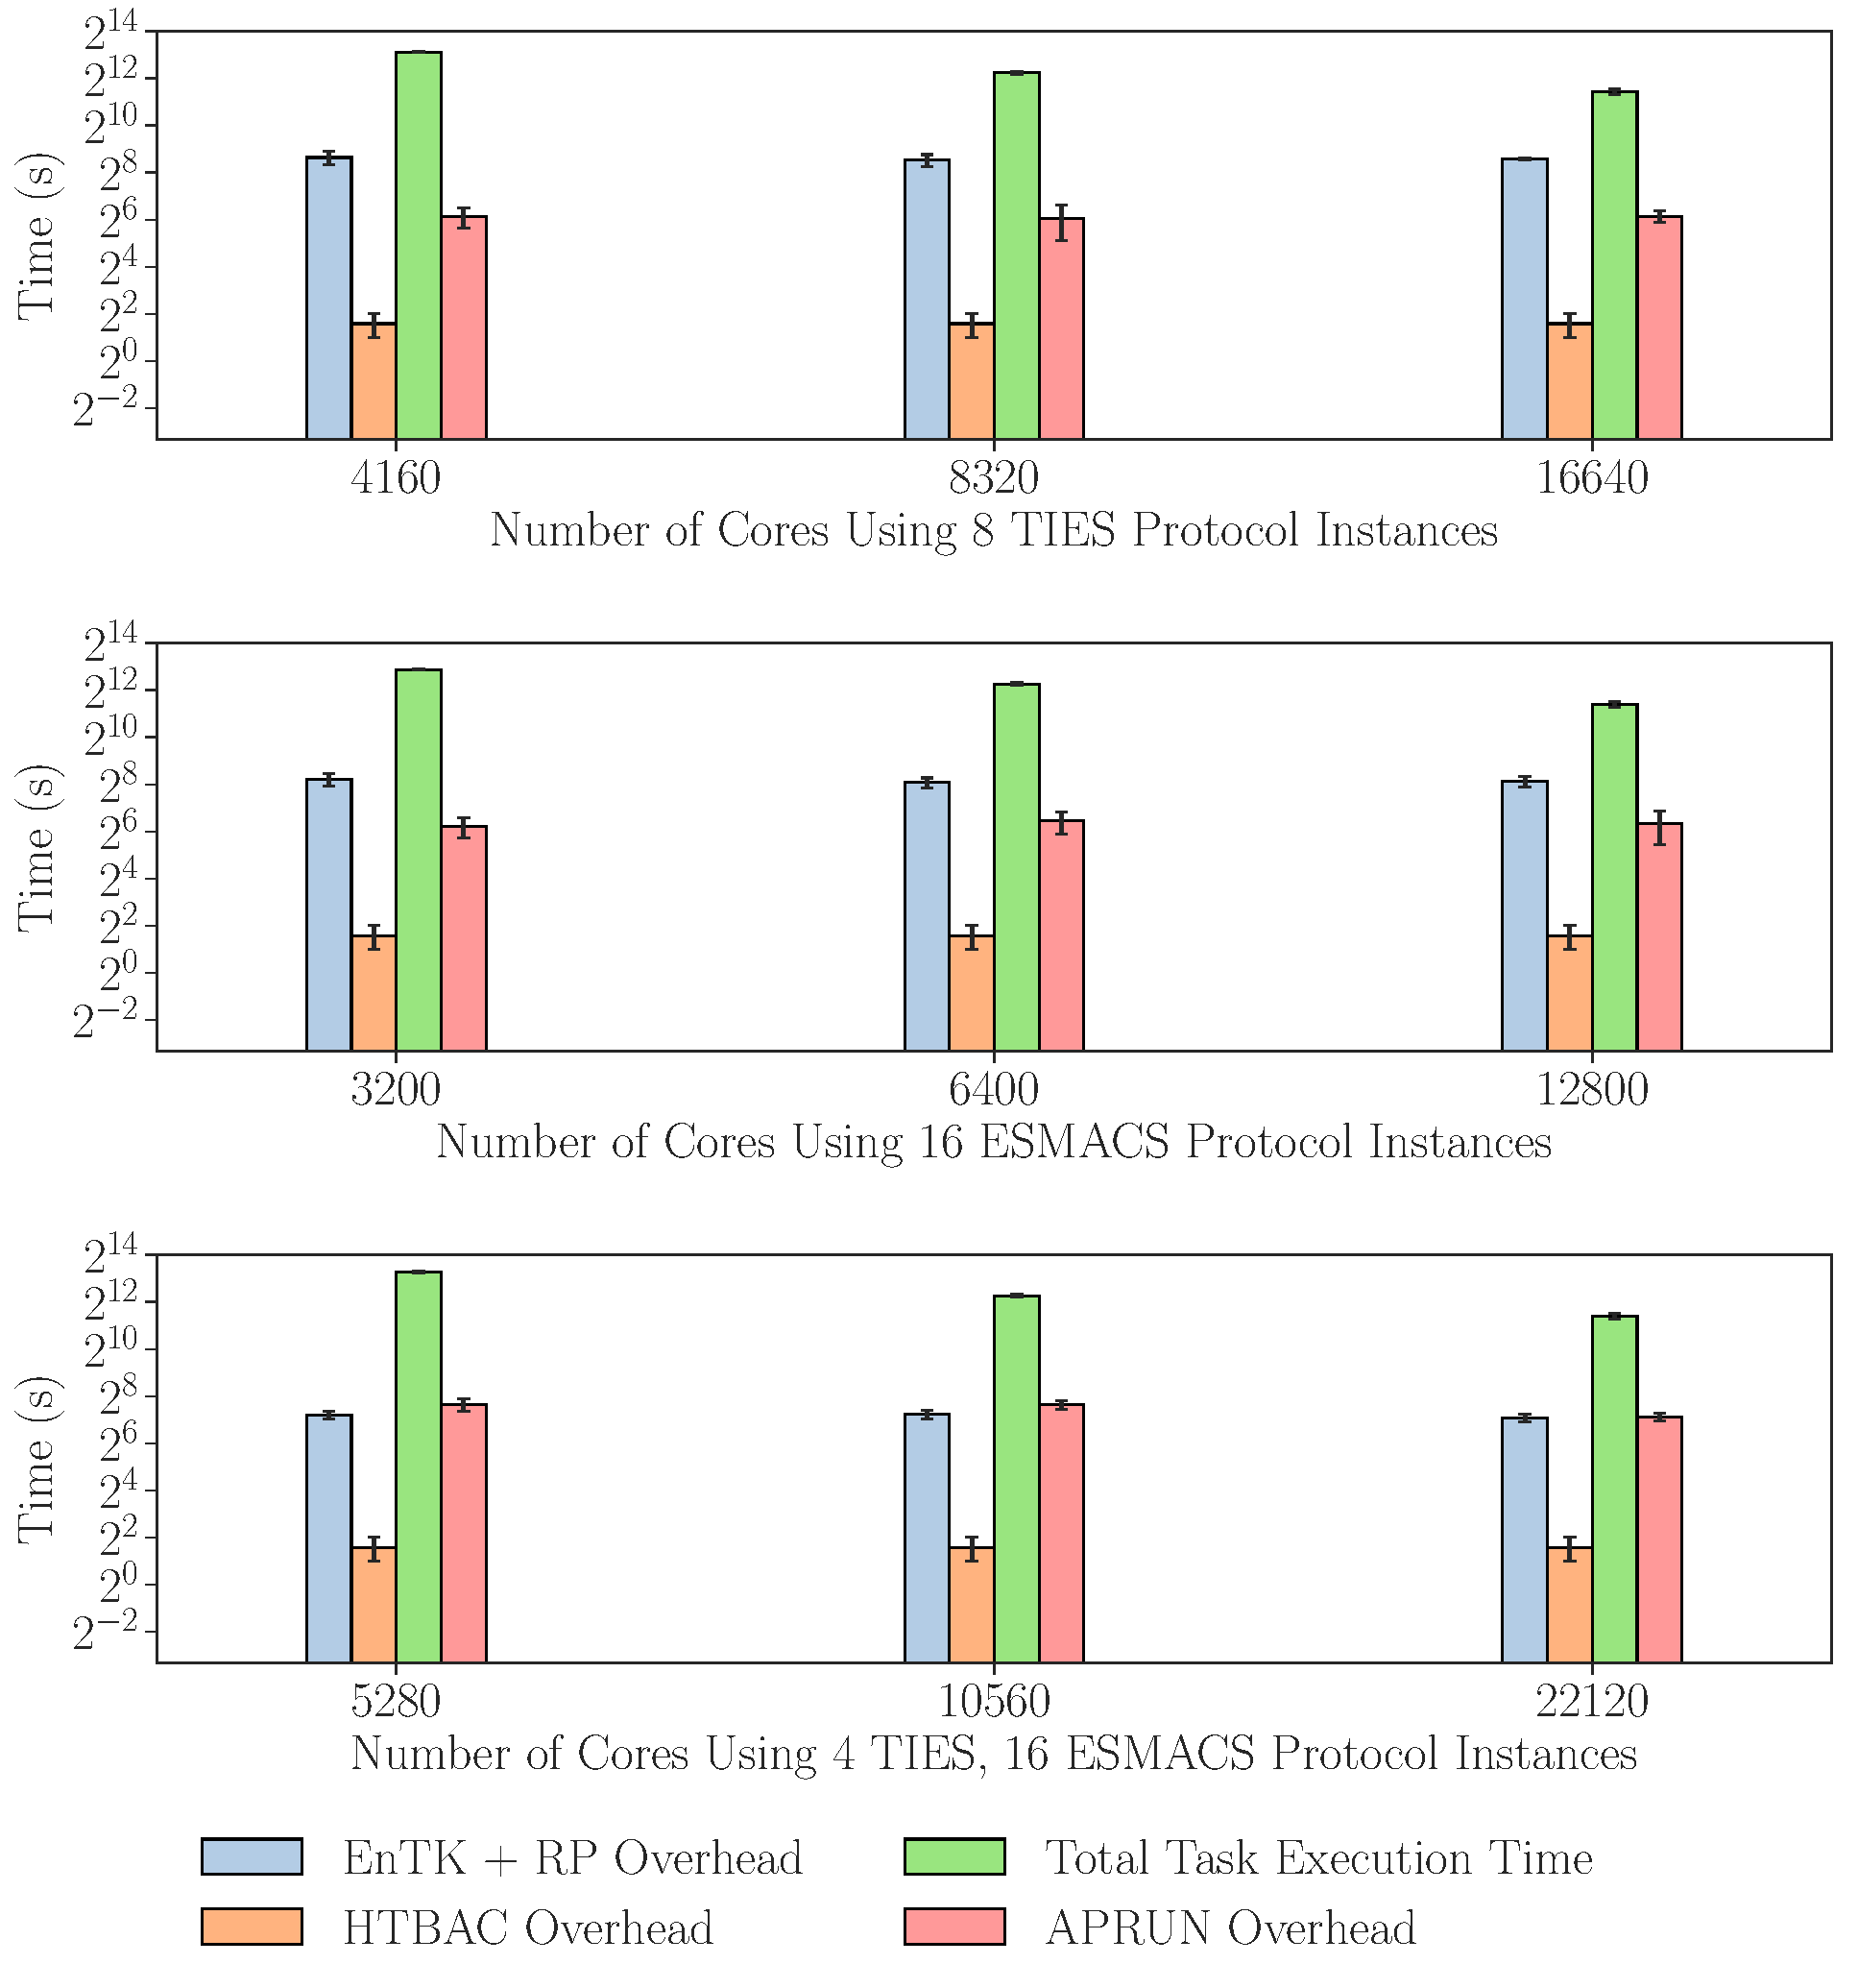
\includegraphics[width=\columnwidth]{figures/ss_all_base2.pdf} 
   \caption{Strong scaling of HTBAC. The number of protocol instances is
    fixed while the number of core increases. Task Execution Time with and
    HTBAC, EnTK+RP, \texttt{aprun} overheads with (a) TIES (Experiment 4) and
    ESMACS (Experiment 5).}\label{fig:ss}
\up{}
\up{}
\up{}
\end{figure}

% \jdnote{this statement is now inconsistent with the performance
% characterization of Ref~\cite{merzky2018} but in
% Ref.~\cite{power-of-many17}, (Power of Many) cites `` EnTK and RP overheads
% mostly depend on the number of managed tasks, not on the size of the pilot
% on which they are executed. This is confirmed for RP in
% Ref.~\cite{merzky2018}." Given that I see the same behavior as what is
% reported in Ref.~\cite{power-of-many17} I used the same
% reference.}\mtnote{Please see discussion on Slack}

% \mtnote{name?}\jdnote{addressed} 
% \mtnote{Are you sure this should not be the `nth experiment
% shows'}\jdnote{addressed}
% \mtnote{See previous comment about application/experiment}\jdnote{fixed}
% \mtnote{add reference to the subsection where generation is defined}

% \mtnote{I am afraid we will need a better explanation for this omission}.
% \jdnote{ Added context. Note about this paragraph: I think the argument
%     about strong scaling only homogeneous protocols can be reduced to the
%     fact that we only show TIES adaptivity. But for the rest of the
%     paragraph, is there merit to put some of these ideas into experiment
%     design?}

% Both applications use the \texttt{BRD4-GSK} physical systems \mtnote{Should
% this detail go in experiment design? This would apply also to the weak
% scaling in the previous section}.
% \jdnote{It's already mentioned in design so we can omit}

% \mtnote{Should we have also a `Weak Scaling Experiments' header? Or maybe
% we should change this one?}
% \jdnote{I changed this subheader to match the subheader +or weak scaling \&
% performance characterization}

% \mtnote{Please add name of the applications}.
% \jdnote{addresed} 

% The objective of strong scaling enables us to examine the properties of 
% adaptive methods. 

% Given the adaptive and nonadaptive methods: if we run the adaptive method
% we achieve time to solution X. With the nonadaptive method, we achieve time
% to solution Y

% We provide the adaptive and nonadaptive methods a fixed amount of
% resources:

% The nonadaptive method runs in time Y with Z accuracy The adaptive method
% runs in time X with N accuracy

% The comparison between weak and strong scaling shows the overhead
% introduced by load balancing and scheduling tasks in multiple generations.

% By design of the TIES protocol, this workload show up to $65 \times 8$
% concurrent tasks, where each task uses 32 cores. The total number of
% concurrent

% \mtnote{See previous comments about terminology}\mtnote{I am not sure I
% understand: are we comparing overheads when weak and strong scaling our
% applications/workflows or are we first measuring the overheads when strong
% scaling and then comparing them to those of weak scaling?}. As we scale the
% number of generation of concurrent tasks executions, we half the resources
% allocated by the pilot \mtnote{this should be explained in the experiment
% setup and design}.

% \mtnote{General note. Experiments about weak and strong scaling show the
% behavior of our software stack with one or more workflows/workloads. The
% question these experiments answer to is: Given a workload/workflow, does
% this software stack scale weakly and/or strongly? This is why, in the
% analysis of our data, we look at the linearity (or lack of thereof) of our
% plots. The analysis of the overhead(s) answer to a different question: What
% part of a measure---e.g., time to completion---depends on the properties of
% an element used to produce that measure---e.g., a component of our software
% stack? Usually, the analysis of the overheads is used to explain why we
% observe lack of scalability (weak or strong) as represented by a
% superlinearity in our plots. The discussion of our experimental results
% should clearly distinguish these questions and properly relate the study of
% scalability to that of overheads. At the moment, our discussion does not do
% all this.}\jdnote{I reduced the discussion of scalability down to the
% properties that relate to contributions of overheads and trends observed in
% TTX.}

% D -------------------------------------------------------------------------
\subsection{Validation}

In order to validate the correctness of the results produced in Experiment
1--5, using HTBAC and the BRD4-GSK physical systems, we compare our results
with those previously published in Wan et al.~\cite{Wan2017brd4}. In this
way, we can confirm that we calculated the correct binding free energies
values.
% \mtnote{NOTE: ESMACS protocol validation is still missing, Kristof is
% working on it.}

We validated our implementation % of the TIES protocol 
selecting a subset of the protein ligand systems used in Wan et
al.~\cite{Wan2017brd4}: ligand transformations 3 to 1, 4, and 7. We then
performed a full simulation on all 3 systems and calculated the binding
affinity using HTBAC.

The results of our experiments, collected in Table~\ref{tab:exp2}, show that
all three $\Delta \Delta$G values are within error bars of the original
study, validating the results we produced with HTBAC.
% and our implementation of the TIES protocol.

\begin{table}
  \centering
  \caption{Validation of HTBAC results against published and experimental
  values}\label{tab:exp2}  
  % \begin{tabular}{l@{\hskip 1in}r@{\hskip 0.2in}r@{\hskip 0.2in}r}
  \begin{tabular}{lrrr}
    \toprule
    System & HTBAC & Wan et al. & Experiment \\
    \midrule
    BRD4 \textbf{3 to 1} & \num{0.39 +- 0.10} &   \num{0.41 +- 0.04} &  \num{0.3 +- 0.09} \\
    BRD4 \textbf{3 to 4} & \num{0.02 +- 0.12} &   \num{0.01 +- 0.06} &  \num{0.0 +- 0.13} \\
    BRD4 \textbf{3 to 7} & \num{-0.88 +- 0.17} &  \num{-0.90 +- 0.08} & \num{-1.3 +- 0.11} \\
    \bottomrule
  \end{tabular}
\up{}
\up{}
\up{}
\end{table}

% HTBAC automates the process of calculating the binding affinity of
% protein-ligand complexes from reading the input to analyzing the final
% results.

% \subsection{Adaptive Experiments}

% The TIES workflow can benefit from an adaptive execution environment to
% improve the efficiency and accuracy of result. In \emph{adaptive
% experiments} we implemented the adaptive quadrature algorithm specifically
% customized for biosimulations.

% In the adaptive workflow, we alter the number of $\lambda$ windows being
% simulated over the course of a protocol instance. The position of new
% $\lambda$ windows depends on the estimated error of the integral measured
% between adjacent windows. Increasing the number of $\lambda$ windows in
% regions of rapid change will increase the accuracy of the overall integral
% to a greater degree than an arbitrarily placed window. In order to
% adaptively add lambda windows, we need access to the $\partial
% U/\partial\lambda$ values during runtime. Therefore, we break down the
% single production simulation stage (S4) \mtnote{I would reference the
% figure with the workflow diagram here} from the nonadaptive workflow into
% multiple smaller stages \mtnote{how many?}, each running for 1 ns. Once
% each simulation is complete within a stage, a decision is made about
% whether more $\lambda$ windows are required, and, if so, where these
% windows should be placed.

% We start out the simulation with 5 replicas of 3 \mtnote{why emphasis for
% 3?}\jdnote{addressed} equally spaced $\lambda$ windows, and equilibrate
% them. Then we repeatedly execute shorter production simulations followed by
% an analysis phase which determines where to place new lambda windows. This
% procedure is repeated until convergence, at which point all concurrent
% simulation are terminated. We define convergence as the point in the
% production-analysis loop at which a desired error threshold is reached.

% The success of this algorithm is determined by the decision where
% additional $\lambda$ windows should be introduced. In adaptive quadrature,
% this decision is made by calculating an error estimate on the integral and
% comparing this estimate to a threshold value. Due to the stochastic nature
% of biosimulations, it is non-trivial to determine this error and, as a
% proof of concept, we simplified this decision to replicate pre-calculated
% results. In future studies, we plan to use a dynamic decision process.

% Inter-node communication introduces a constraint on the number of new
% $\lambda$ windows that can be added at each iteration. Simulations must run
% on an integer number of nodes to reduce the overhead of inter-node
% communication. This means that the number of new $\lambda$ windows (i.e.,
% the number of simulations) \emph{has} to be either doubled or left
% unchanged. If the number of windows is doubled, the number of nodes per
% simulation can be halved automatically. Our algorithm loops through the
% current $\lambda$ window pairs until this criterion is reached, forcefully
% adding more windows when needed.

% I don't think we need this equation here, it's too trivial.
% \begin{flalign} L &= \{ x_i: x_i\in[0,1]\; and\; x_{i+1} = x_i + \delta \},
% where\ \delta\ is\ 0.5. %&$$L=\{ x_i: x_i\in[0,1]\; and\; x_{i+1} = x_i +
% \delta \}$$%, where $\delta$ is $0.1$.
% \end{flalign}

% For every $\lambda$ window we initialize with five replicas therefore
% yielding a total of 15 tasks. We run 15 tasks for stages $S1$ through
% $S4.1$. Between stages $S4.1$ and $S4.3$ the number of $\lambda$ windows
% doubles for every stage, which doubles the total number of tasks. The last
% production simulation stage, $S4.4$, runs for the remaining 2 ns durations.

% Our experiments implement adaptive change in the $\lambda$ windows sampled
% and not the timing of execution. In this way, we introduce only a single
% \mtnote{additional?} degree of freedom relative to \mtnote{compared to?}
% our baseline ``non-adaptive" experiments. HTBAC provides the functional
% capability to adaptively determine the time at which the $\lambda$ windows
% are chosen. However, in this paper we do not investigate the impact of such
% adaptivity, as the objective is to determine the feasibility of adaptive
% execution and the scientific merit of adaptive decision making.

% \begin{figure}
%   \centering
%     \includegraphics[width=\columnwidth]{figures/adaptive_vs_nonadaptive_ps
%     eudo.pdf}
%     \caption{Illustrating the adaptive vs. non-adaptive workflow given the
%     same number of core hours}
% \label{fig:adaptive_vs_nonadaptive_TIES}
% \end{figure}

% E -------------------------------------------------------------------------
\subsection{Adaptive Experiments}

% \jhanote{On looking at this afresh, this whole paragraph should either be
% zapped for it does not belong here but in an earlier section} \sout{Even at
% small scale it is hard to implement adaptive al- gorithms that use common
% molecular dynamics simulations engines (e.g., NAMD, Gromacs, Amber). This
% is in part because of the way the scientist interacts with these codes. The
% user hand- writes a configuration file and, together with the physical
% system description (topology, PDB), passes it to a binary executable,
% waiting for the simulation to end before analyzing the results. There is a
% disconnect between running the simulation and analysis, i.e. the
% intermediate results have no influence over the simulation parameters
% \emph{after} it has been started. Therefore, certain decisions, like number
% of time steps, $\lambda$ window placement have to be made \emph{a priori},
% and the continuous accumulation of results can, by definition, have no
% effect of these parameters.}

% \jhanote{This discussion needs more care: adaptive algorithms are difficult
% to implement at scale. That is why we have fewer adaptive algorithms than
% one might suspect. The opening line says the cause of the lack of
% adaptivity is  the way they are implemented.}\kfnote{I was trying to
% describe this smaller problem, not related to scale, just adaptivity. I
% modified the sentence to reflect this.}

The design of HTBAC permits enhancing protocols while continuing to use
``static'' simulation engines. To this end, we implemented two adaptive
methods using HTBAC: adaptive quadrature and adaptive termination. Both of
these methods use the features of adaptivity offered in HTBAC to scale to
large number of concurrent simulations and to increase convergence rate and
obtain more accurate scientific results.

% \jhanote{Once again, we need to be careful: there is conflation between
% cause and effect. Adatpvitiy is not a principle in of itself so has not
% intrinsic value standalone. what is important is faster convergence and
% more accurate results. adaptivity is one route to obtain them. The way the
% previous sentence is written conflates effect with
% driver.}\kfnote{Rephrased to reflect this.}

% \jhanote{adaptive quadrature is raised several times it isn't describe
% anywhere}\kfnote{it is in previous sections, no?}\jhanote{Its probably
% fine. A picky reviewer will complain that we talk about how it is used, but
% not why it is used? Or which type of adaptive quadrature}

The aim of introducing adaptive quadrature for alchemical free energy
calculation protocols (e.g., TIES) is to reduce time to completion while
maintaining (or increasing) the accuracy of the results. Time to completion
is measured by the number of core hours consumed by the simulations. Accuracy
is defined as the error with respect to a reference value, calculated via a
dense $\lambda$ window spacing (65 windows). This reference value is used to
establish the accuracy of the non-adaptive protocol (which has 13 $\lambda$
windows) and the adaptive protocol (which has a variable number of $\lambda$
windows, determined at run time).

One of the input parameters of the adaptive quadrature algorithm is the
desired acceptable error threshold of the estimated integral. We set this
threshold to the error of the non-adaptive algorithm calculated via the
reference value. The algorithm then tries to minimize the number of $\lambda$
windows constrained by the accuracy requirement.

\begin{figure}
  \begin{tikzpicture}
\begin{axis}[
  ybar,
  ymin=0,
  ylabel=Error (kcal/mol),
  x tick label style  = {text width=1.5cm,align=center},
  symbolic x coords={PTP1B L1-L2,PTP1B L10-L12,TYK2 L7-L8,TYK2 L4-L9,MCL1 L32-L38}
  ]
  
\addplot+[color=Orchid] table [x=System, y=Non-adaptive error, col sep=comma] {figures/savings.csv};

\addplot+[color=YellowGreen] table [x=System, y=Adaptive error, col sep=comma] {figures/savings.csv};


\legend{Non-adaptive,Adaptive}
  
\end{axis}
\end{tikzpicture}%
%
%
\begin{tikzpicture}
\begin{axis}[
  ybar,
  ymin=0,
  ylabel=Resource consumption (CPU-hours),
  x tick label style  = {text width=1.5cm,align=center},
  symbolic x coords={PTP1B L1-L2,PTP1B L10-L12,TYK2 L7-L8,TYK2 L4-L9,MCL1 L32-L38}
  ]
  
\addplot+[color=Orchid] table [x=System, y=Non-adaptive cpuh, col sep=comma] {figures/savings.csv};

\addplot+[color=YellowGreen] table [x=System, y=Adaptive cpuh, col sep=comma] {figures/savings.csv};


\legend{Non-adaptive,Adaptive}
  
\end{axis}
\end{tikzpicture}
%
  \caption{Quantifying the benefits of the adaptive quadrature simulations.
  (top) The error of the adaptive run is reduced for all 5 test systems,
  sometimes by a significant amount. It has been shown that reproducibility
  of free energy calculations can be achieved up to
  \SI{0.2}{\kilo\calorie\per\mole}~\cite{Loeffler2018}. The adaptive
  algorithm brings down the error of the nonadaptive simulations below this
  threshold, ensuring that results are also reproducible. (bottom) Resource
  consumption is reduced, except for one of the systems, where the low error
  threshold required more $\lambda$ windows.}\label{fig:savings}
\up{}
\up{}
\end{figure}

Table~\ref{tab:adapquad} shows the results of running adaptive quadrature on
5 protein ligand systems, comparing the Total Task Execution Time and
accuracy versus the non-adaptive case. The number of lambda windows are
reduced on average by \SI{32}{\percent}, hence reducing Total Task Execution
Time by the same amount. The error on the adaptive results is also decreased,
on average by \SI{77}{\percent} (see fig.~\ref{fig:savings}). More
importantly, the error on all of the systems are reduced to below
\SI{0.2}{\kilo\calorie\per\mole}, which has recently been shown to be the
upper bound of reproducibility across different simulation
engines~\cite{Loeffler2018}.

The Total Task Execution Time of the TYK2 L7--L8 system has increased for the
adaptive run by 1 $\lambda$ window, compared to the non-adaptive case. This
is due to the non-adaptive error being very low, and matching that same
accuracy required the use of a large number of windows. Nonetheless due to
the efficient placing of the windows, the accuracy of the free energy still
increased by \SI{40}{\percent}.

\begin{table*}
  \caption{Comparing results of adaptive, non-adaptive and reference
  runs.}\label{tab:adapquad}
  \begin{tabular}{lSSSSS[table-format=5.1]S[table-format=5.1]}
    \toprule
    {System}                               & 
    {\makecell{Ref $\Delta \Delta$G \\ (\si{\kilo\calorie\per\mole})}}  &
    {Non-adaptive $\Delta \Delta$G}        &
    {Adaptive $\Delta \Delta$G}            &
    {Num. of $\lambda$ windows}            &
    {Decrease in TTX}       &
    {Increase in accuracy}                 \\
    \midrule
    {PTP1B L1-L2}   & 
    -58.51 & 
    -57.87(64) & 
    -58.60(9) & 
    10 & 
    23\si{\percent} & 
    86\si{\percent} \\
    %
    {PTP1B L10-L12} & 
    1.83   & 
    2.05(22) & 
    1.94(7)  & 
    6  & 
    54\si{\percent} &
    68\si{\percent} \\
    %
    {MCL1  L32-L38} & 
    2.13   & 
    2.33(20) & 
    2.14(1)      & 
    7  & 
    46\si{\percent} & 
    95\si{\percent} \\
    %
    {TYK2  L4-L9}   &
    -28.69 & 
    -28.25(44) & 
    -28.67(1)  & 
    7  & 
    46\si{\percent} & 
    98\si{\percent} \\
    %
    {TYK2  L7-L8}   & 
    4.97   & 
    4.92(5) & 
    5.00(3)      & 
    14 &  
    -8\si{\percent} & 
    40\si{\percent} \\
    \bottomrule 
  \end{tabular}
\end{table*}

% \jhanote{This para is difficult to parse. How does one appreciate the
% iteration count? Needs complete rewrite.} \kfnote{rewrote}
Fig.~\ref{fig:adapconv} compares the error on the adaptive and non-adaptive
simulations as a time series plot. As fewer lambda windows are calculated the
adaptive algorithm uses less resources. Remarkably, the error is drastically
reduced as the windows are placed adaptively to capture the changes in
function.

\begin{figure}
  \begin{tikzpicture}
\begin{axis}[
  title style={align=center},
  title={Observed accuracy of adaptive vs. non-adaptive workflows\\for same simulation duration ({\SI{6}{\nano\second}}) },
  no markers,
  every axis plot/.append style={ultra thick},
  xlabel=Resource consumption (CPU-hours),
  ylabel=Error (kcal/mol),
  scaled ticks=false,
  yticklabel style={
  /pgf/number format/precision=3,
  /pgf/number format/fixed},
  scale=0.85,
  ]
  
  
\addplot+[color=Orchid, smooth] table [x=Resource consumption, y=Non-adaptive error, col sep=comma] {figures/non_adaptive_accuracy.csv};

\addplot+[color=YellowGreen, smooth] table [x=Resource consumption, y=Adaptive error, col sep=comma] {figures/adaptive_accuracy.csv};

\legend{Non-adaptive,Adaptive}

\draw[densely dotted, color=gray] (10586.058921984,0.049299384672436553) -- (12000,0.049299384672436553);
\draw[densely dotted, color=gray] (8143.1222476800012,0.0015858767437348931) -- (12000,0.0015858767437348931);

\draw[densely dotted, color=gray] (10586.058921984,0.08) -- (10586.058921984,-0.025);
\draw[densely dotted, color=gray] (8143.1222476800012,0.08) -- (8143.1222476800012,-0.025);
\draw[->] (10586.058921984,0.075) -- (8143.1222476800012,0.075) ;
\node[align = right] at (8700, 0.115) {Resource\\consumption\\decrease};

\node at (9200, 0.025) {\contour{white}{Error decrease}};
\draw[->] (11500,0.049299384672436553) -- (11500,0.0015858767437348931) ;


  
\end{axis}
\end{tikzpicture}

  \caption{Plot of the error estimate as a function of the resource
  consumption, comparing the adaptive and nonadaptive simulations. The error
  estimate converges for both simulations but the window placement of the
  adaptive simulation considerably lowered the error.}\label{fig:adapconv}
\up{}
\up{}
\end{figure}

% \jhanote{I would not use ``protocol''} \kfnote{method?}

Adaptive quadrature is specific to alchemical free energy calculations.
\emph{Adaptive termination}, the second adaptive method implemented in HTBAC,
offers dynamic termination for any simulation protocol that has as its aim
the prediction of an observable value. The protocol monitors the convergence
of the observable as the simulation progresses, and stops the execution when
a criterion has been met. Non-adaptive protocols usually have a predefined
simulation time, set based on the assumption that the simulation will
converge by that time. This means that in practical examples the simulation
might have converged before the predefined time interval.

In the original TIES protocol the production part of the simulation has to be
run for \SI{4}{\nano\second} and the results are analyzed thereafter. This
assumes that all systems need this simulation time for the results to
converge. In reality, certain systems could converge faster, therefore one
can terminate the simulation before the static \SI{4}{\nano\second} end. This
would lead to faster time to insight and less compute resources consumed.
Adaptive termination was implemented in HTBAC by having a checkpoint every
$\tau = \SI{0.5}{\nano\second}$ in the simulation. Fig.~\ref{fig:termination}
shows how the observable for a specific simulation changes as a function of
resource consumption. At every checkpoint the convergence is evaluated, and
the simulation is indeed terminated earlier than the non-adaptive protocol
would suggest. Table~\ref{tab:adapterm} shows results that the adaptively
terminated TIES protocol saves compute resources and reduces time to insight
on average by \SI{16}{\percent} for the physical systems tested.

\begin{figure}
  \begin{tikzpicture}
\begin{axis}[
  height=5cm,
  width=\columnwidth,
  every axis plot/.append style={ultra thick},
  xlabel=Resource consumption (CPU-hours),
  ylabel=$\Delta$G (kcal/mol),
  scaled ticks=false,
  yticklabel style={
  /pgf/number format/precision=3,
  /pgf/number format/fixed},
  xmin=3533.3975040000005,
  xmax=12000,
  ymax=4.85,
  ]
  
  
\addplot+[no markers, color=Orchid, smooth, error bars/.cd, y dir=both,y explicit, error mark=none, error bar style={draw=gray}] table [x=Resource consumption, y=dG, col sep=comma] {figures/adaptive-termination-begin.csv};

\addplot [only marks, mark=|, mark options={color = OliveGreen, mark size = 5pt, thick}] coordinates {(4416.746880000001,4.451008938594887) (5300.096256000001,4.490752904442608) (6183.445632000001,4.543730747316334) (7066.795008000001,4.5784909284966355) (7950.144384000001,4.586120549368642) (8833.493760000001,4.5843340530391075) (9716.843136000001,4.577994475375011) (10600.192512000001,4.571614686607193) };

\addplot+[densely dashed, semithick, no markers, color=Orchid, smooth, error bars/.cd, y dir=both,y explicit, error mark=none, error bar style={draw=gray}] table [x=Resource consumption, y=dG, col sep=comma] {figures/adaptive-termination-end.csv};

\legend{Observable, Checkpoint}

% \draw[densely dotted, color=gray] (10586.058921984,0.049299384672436553) -- (12000,0.049299384672436553);
% \draw[densely dotted, color=gray] (8143.1222476800012,0.0015858767437348931) -- (12000,0.0015858767437348931);
% 
\draw[densely dotted, color=gray] (7950.144384000001,4.8) -- (7950.144384000001,4.4);
% \draw[densely dotted, color=gray] (8143.1222476800012,0.08) -- (8143.1222476800012,-0.025);
% \draw[->] (10586.058921984,0.075) -- (8143.1222476800012,0.075) ;
% \node[align = right] at (8700, 0.115) {Resource\\consumption\\decrease};
% 
\node[align = right] at (6800, 4.7) {Adaptively\\terminated};

\draw[densely dotted, color=gray] (10600.192512000001,4.8) -- (10600.192512000001,4.4);

\node[align = right] at (9300, 4.5) {Non-adaptive\\protocol end};


% \draw[->] (11500,0.049299384672436553) -- (11500,0.0015858767437348931) ;
% 
  
\end{axis}
\end{tikzpicture}

  \caption{Plot of the free energy as a function of the resources consumed
  (hence simulation time). The adaptive termination algorithm checks the
  convergence of the observable every $\tau = \SI{0.5}{\nano\second}$ and if
  the threshold (\SI{0.01}{\kilo\calorie\per\mole}) has been met, terminates
  the simulation.}\label{fig:termination}
\end{figure}

\begin{table}
  \caption{Simulation time of non-adaptive and adaptively terminated runs for
  a given convergence criterion\jhanote{Reviwer will want to know what happens with
  remaining two candidates?}\kfnote{Results are in the table for all the
  systems.}\jhanote{Sorry wrong caption. Moved to table IV.}}\label{tab:adapterm}
  \centering
  \begin{tabular}{lSSS[table-format=5.1, table-column-width=2cm]}
    \toprule
    {System}                               & 
    {Non-adaptive}      &
    {Adaptive}          &
    {Decrease in TTX}       \\
    \midrule
    {PTP1B L10-L12} & 
    6.0\si{\nano\second}   & 
    5.0\si{\nano\second}   & 
    16.7\si{\percent} \\
    %
    {TYK2 L4-L9}   &
    6.0\si{\nano\second} & 
    5.5\si{\nano\second} & 
     8.3\si{\percent} \\
    %
    {TYK2 L7-L8}   & 
    6.0\si{\nano\second}  & 
    4.5\si{\nano\second} & 
    25.0\si{\percent} \\
    \bottomrule 
  \end{tabular}
\up{}
\up{}
\end{table}

% \kfnote{Move this to algorithm description} In previous studies \cite{} the
% error estimation during the adaptive algorithm is done by calculating the
% integral estimate using two methods, one lower and one higher in
% complexity, then the difference between the two can constitute as a rough
% estimate of the error on that interval.
